Para realizar la pantalla de supervisión, control y adquisición de datos operador (SCADA) se utilizó el software iFix perteneciente al grupo \textbf{General Electric}.

El sistema HMI creado (Figura \ref{fig:scada1}) se dividió en las siguientes secciones:
\begin{itemize}
	\item Esquemático del circuito hidráulico físico con las variables de presión y caudal en tiempo real.
	\item Valores de funcionamiento del motor obtenidos por el variador de velocidad.
	\item Alarmero, dónde se observa de forma visual valores críticos alcanzados en el sistema.
	\item Indicador de modo de funcionamiento físico o remoto.
	\item Modo de control a lazo abierto o lazo cerrado.
	\subitem Para el modo de lazo cerrado se creó una ventana individual para cada sistema de presión y caudal.
	\item Pantalla para observar gráficos en tiempo real dónde se divide según la variable a observar, con botones para abrir el control PID del sistema.
	\item Pantalla donde se observa datos históricos y se puede generar un archivo \textit{.txt} con la información de la variable elegida en un determinado período de tiempo.
\end{itemize} 

\begin{figure}[htb]
	\centering
	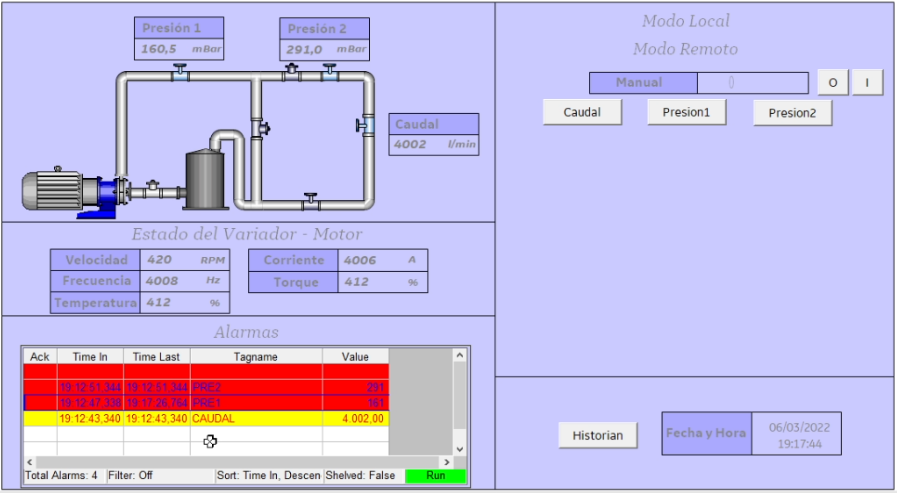
\includegraphics[scale=0.5]{scada1.png}
	\captionof{figure}{Pantalla SCADA}
	\label{fig:scada1}
\end{figure}


\subsubsection{Comunicación SCADA- Computadora}
Para realizar la configuración de cada ícono de la pantalla SCADA con su respectiva variable, se debió crear un MBE Driver (Figura \ref{fig:mbe}) dónde se estipula la dirección IP y el mapa de memoria con sus respectivas secciones que luego serán utilizadas por el DataBase (Figura \ref{fig:database}). 

Una vez creado el MBE Driver se debe generar la tabla \textit{DataBase} en dónde estará el nombre, dirección IP, tipo de elemento, descripción, alarma asociada, entre otros puntos de cada elemento.

La lista se encontrará unificada con las direcciones de \textit{UnityPro} (Tabla..\fcolorbox{red}{yellow}{..}).

\begin{figure}[h]
	\centering
	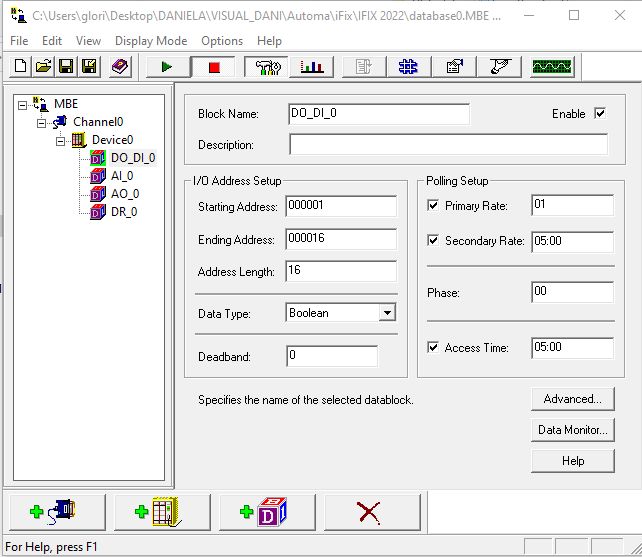
\includegraphics[scale=0.6]{mbe.png}
	\captionof{figure}{Configuración MBE}
	\label{fig:mbe}
\end{figure}
\begin{figure}[h]
	\centering
	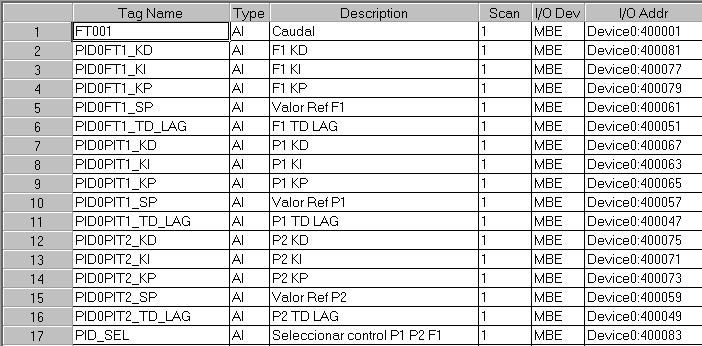
\includegraphics[scale=0.6]{database.png}
	\captionof{figure}{Configuración MBE}
	\label{fig:database}
\end{figure}


\paragraph{Pruebas mediante ModSim}
Para realizar pruebas intermedias antes de unir SCADA con el programado para el PLC se utilizó el software ModSim, dónde se generó los distintos mapas de memoria utilizados y allí se podían modificar variables para observar el correcto funcionamiento de distintos elementos en el HMI.

\begin{figure}[htb]
	\centering
	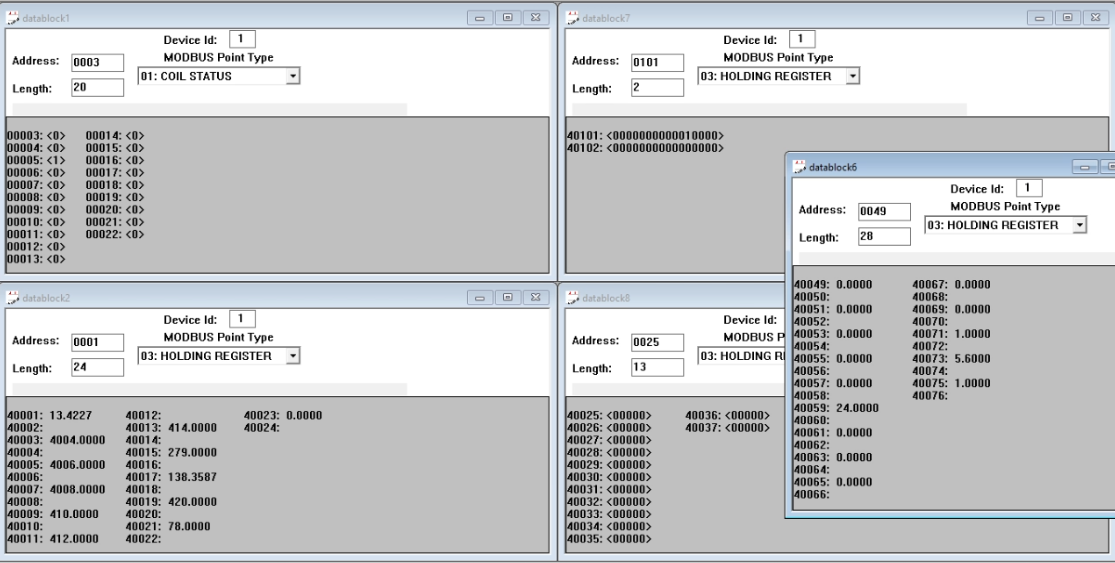
\includegraphics[scale=0.5]{modsim1.png}
	\captionof{figure}{ModSim}
	\label{fig:modsim1}
\end{figure}



\subsubsection{Alarmas}
Dentro de la pantalla principal es posible observar el alarmero. Estas alarmas están compuestas por las variables de la siguiente \fcolorbox{red}{yellow}{tabla} con sus respectivos valores y prioridades.\\
\fcolorbox{red}{yellow}{Poner lista que esta en drive}
\subsubsection{iHistorian}
\begin{figure}[htb]
	\centering
	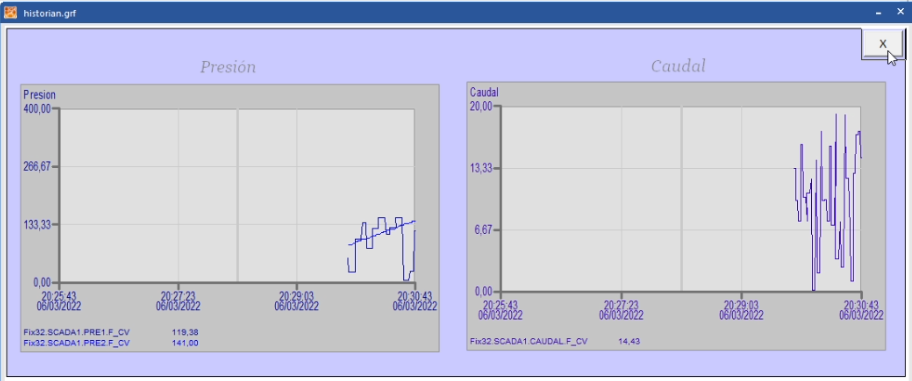
\includegraphics[scale=0.5]{scada3.png}
	\captionof{figure}{Pantalla SCADA}
	\label{fig:scada3}
\end{figure}

